\documentclass[11pt,aspectratio=43]{beamer}
\usepackage[utf8]{inputenc}
\usepackage{amsmath, amsfonts, amssymb, amsthm}
\usepackage[T1]{fontenc}
\usepackage{lmodern}
\usepackage{xcolor}
\usepackage{setspace}
\usepackage{booktabs}
\usepackage{multirow}
\usepackage{graphicx}
\usepackage{tikz}
% \usetikzlibrary{decorations}
\usetikzlibrary{decorations.pathreplacing}
\usepackage{ulem}
\usepackage{hyperref}
\usepackage{booktabs}
\usepackage{babel}
\usepackage{makecell}
\usepackage[para,online,flushleft]{threeparttable}
\usepackage{pdfpages}
\usepackage{tcolorbox}
\usepackage{bm}
\usepackage{appendixnumberbeamer}
\usepackage{natbib}
\usepackage{caption}
\captionsetup[figure]{labelformat=empty}% redefines the caption setup of the figures environment in the beamer class.
\usetheme[compress]{Boadilla}
\usecolortheme{default}
\useoutertheme{miniframes}
\usefonttheme[onlymath]{serif}

\newcommand{\jump}[2]{\hyperlink{#1}{\beamerbutton{#2}}}
\newcommand{\orange}[1]{\textcolor{orange}{#1}}
\newcommand{\red}[1]{\textcolor{red}{#1}}

\setbeamertemplate{itemize item}{\raisebox{0.1em}{\scalebox{0.7}{$\blacksquare$}}}
\setbeamertemplate{itemize subitem}[circle]
\setbeamertemplate{itemize subsubitem}{--}
\setbeamercolor{itemize item}{fg=black}
\setbeamercolor{itemize subitem}{fg=black}
\setbeamercolor{itemize subsubitem}{fg=black}
\setbeamercolor{item projected}{bg=darkgray,fg=white}
\definecolor{blue}{rgb}{0.2, 0.2, 0.7}
\setbeamercolor{alerted text}{fg=blue}
\setbeamertemplate{enumerate items}[circle]


\setbeamertemplate{headline}{}

%==========================================
\let\olditemize=\itemize
\let\endolditemize=\enditemize
\renewenvironment{itemize}{\olditemize \itemsep1em}{\endolditemize}
\let\oldenumerate=\enumerate
\let\endoldenumerate=\endenumerate
\renewenvironment{enumerate}{\oldenumerate \itemsep1em}{ \endoldenumerate}

\DeclareMathOperator*{\argmax}{\arg\!\max}
\DeclareMathOperator*{\E}{\mathbb{E}}
\DeclareMathOperator*{\var}{\rm Var}
\DeclareMathOperator*{\cov}{\rm Cov}

\theoremstyle{definition}
\newtheorem{assume}{Assumption}
\newtheorem{lem}{Lemma}
\newtheorem{proposition}{Proposition}
\newtheorem{thm}{Theorem}
\newtheorem{corol}{Corollary}

\begin{document}
    \title[Lecture 12]{Lecture 12: Two-Period Consumer Problem}
    \author[Hui-Jun Chen]{Hui-Jun Chen}
    \institute[OSU]{The Ohio State University}
    % \date{\today}
    \date{\today}
    \setbeamertemplate{navigation symbols}{}
    \setstretch{1.2}

%-------------------------------------------------------
{
%	\usebackgroundtemplate{\includegraphics[width=1\paperwidth]{../EveningSky_cropped_edit43_bright.jpg}}
    \begin{frame}
% \vspace{3em}
        \centering
%		{\footnotesize 	ECON 4002 Intermediate Macroeconomic Theory}
        \maketitle
% \vspace{-1.5em}
% \centering
% \includegraphics[width=0.55\linewidth]{Pictures/houses.jpeg}


    \end{frame}
}

% -------------------------------------------
\setbeamertemplate{headline}
{
\setbeamercolor{section in head/foot}{fg=black, bg=white}
\vskip1em \tiny \insertsectionnavigationhorizontal{1\paperwidth}{\hspace{0.50\paperwidth}}{}
}
%------------------------------------------

\section{Budget}
\label{sec:Budget}


\begin{frame}{Variables and Notation}
\label{slide:Variables_and_Notation}
    Assume that consumer do NOT make consumption-leisure decision, but receive endowment of \alert{non-labor income} $ y $ and subject to \alert{lump-sum tax} $ t $.
    \begin{itemize}
        \item $ y $ \& $ t $: today (date 0), and $ y' $ \& $ t' $: tomorrow (date 1)
        \item in general, having a prime ``$'$'' represents tomorrow
    \end{itemize}
    If there's a \alert{saving technology} exists (may not be available!), then consumer saves $ s $ today for tomorrow consumption, i.e.,
    %
    \begin{equation*}
       c + s \le y - t
    ,\end{equation*}
    %
    where $ s > 0 $ represents ``saver'', and $ s < 0 $ represents ``borrower''.
\end{frame}

\begin{frame}{Savings and the Credit Market}
\label{slide:Savings_and_the_Credit_Market}
    Buying/selling \alert{Bonds} are the way to achieve saving $ s $.
    \begin{itemize}
        \item lenders/savers \red{buy} bonds; borrowers \red{sell} bonds.
    \end{itemize}
    Consumer will get $ 1+r $ unit of consumption goods tomorrow if he/she buys $ 1 $ unit of bond today, and thus tomorrow's budget constraint is
    %
    \begin{equation*}
       c'= y' - t'+ ( 1+r )s
    ,\end{equation*}
    %
    where $ r $ is the (net) \alert{real interest rate}, and ``$=$'' since \alert{no date 2}.
    \begin{itemize}
        \item \alert{relative price} of consumption between today and tmw: $ \frac{1}{1+r} $
        \item no default on bonds
        \item no middle man: bonds are trade directly between savers and borrowers
    \end{itemize}
\end{frame}

\begin{frame}{The Lifetime Budget Constraint}
\label{slide:The_Lifetime_Budget_Constraint}
    %
    \begin{align*}
        \text{Date 0}: \quad
            & c + s = y - t
        \\
        \text{Date 1}: \quad
            & c' = y' - t' + ( 1+r )s
        \\
        \text{Saving}: \quad
            & \Rightarrow s = \frac{c' - y' + t'}{1+r}
        \\
        \text{Plug saving back to Date 0}: \quad
            & c + \frac{c' - y' + t'}{1+r} = y - t
        \\
        \text{Rearrange}: \quad
            & \underbrace{%
                c + \frac{c'}{1+r}
              }_{\text{(1)}}
                =
              \underbrace{%
                y - t + \frac{y' - t'}{1+r};
              }_{\text{(2)}}
    \end{align*}
    %
    \begin{itemize}
        \item (1): \alert{present value of total lifetime consumption} (choice by consumer)
        \item (2): \alert{present value of total lifetime net worth}, also called $ we $ (fixed).
    \end{itemize}
\end{frame}

\begin{frame}{Numerical Example of Present Value}
\label{slide:Numerical_Example_of_Present_Value}
    Suppose we have data:
    \begin{tabular}{| c | c | c | c | c | }
        \hline
        $ y $
            & $ y' $
            & $ t $
            & $ t' $
            & $ r $
        \\
        \hline
        \hline
        $ 110 $
            & $120$
            & $ 20 $
            & $ 10 $
            & 0.1
        \\
        \hline
    \end{tabular}

    The face value of the net worth is
    %
    \begin{equation*}
        y - t + y' - t' = 110 - 20 + 120 - 10 = 200
    \end{equation*}
    %
    The present value of lifetime the net worth is
    %
    \begin{equation*}
        y - t + \frac{y' - t'}{1+r} = 110 - 20 + \frac{120 - 10}{1.1} = 190
    \end{equation*}
    %
    Future part has discounted $ 10\% $ to be evaluated in consumption goods today.
\end{frame}



\begin{frame}{Visualization: Lifetime Budget Constraint}
\label{slide:Visualization__Lifetime_Budget_Constraint}
    \begin{columns}
        \begin{column}{0.5\textwidth}
            \begin{figure}
                \caption{\scriptsize Figure 9.1 Consumer’s Lifetime Budget Constraint}
                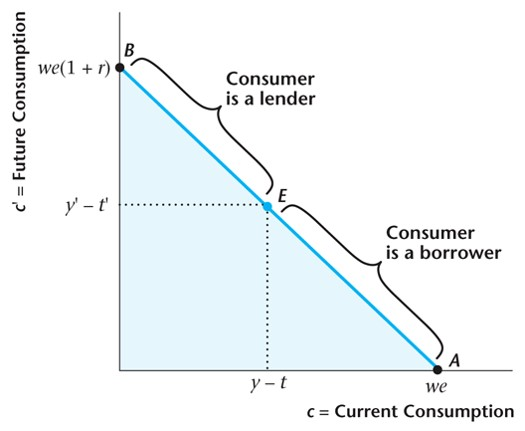
\includegraphics[width=\textwidth]{./figures/Figure9_1.jpg}
            \end{figure}
        \end{column}
        \begin{column}{0.5\textwidth}
            On $ ( C, C' ) $ plane, $ \because $ substitution between current and future consumption.
            %
            \begin{equation*}
                 c' = \underbrace{we ( 1+r )}_{\text{y-intercept}} \underbrace{-( 1+r )}_{\text{slope}} c
            \end{equation*}
            %
            \begin{itemize}
                \item \textit{E}: \alert{endowment point}, where $ c = y-t $, and $ c' = y' - t' $.
                \item $\overline{BE}$: lending, give up $ c $ for $ c' $
                \item $\overline{AE}$: borrowing, the opposite
            \end{itemize}
        \end{column}
    \end{columns}
\end{frame}

\section{Preference}
\label{sec:Preference}

\begin{frame}{Consumer Preference in Two-Period Model}
\label{slide:Consumer_Preference_in_Two_Period_Model}
Since it is substitution between $ ( c, c' ) $, utility is $ U( c, c' ) $, so
\begin{columns}
    \begin{column}{0.4\textwidth}
        \begin{figure}
            \caption{\scriptsize Figure 9.2  A Consumer’s Indifference Curves}
            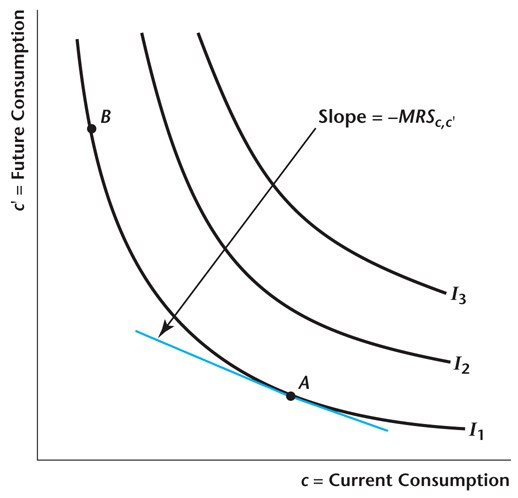
\includegraphics[width=\textwidth]{./figures/Figure9_2.jpg}
        \end{figure}
    \end{column}
    \begin{column}{0.6\textwidth}
        \begin{enumerate}
            \item \textbf{monotonicity}: more is preferred
            \begin{itemize}
                \item slope $ = -MRS_{c, c'}$ (substitution)
                \item $ U( I_{3} ) > U( I_{2} ) > U( I_{1} ) $
            \end{itemize}
            \item \textbf{convexity}: diversity is preferred
            \begin{itemize}
                \item Is bow in towards the origin
                \item \alert{consumption smoothing}: preferred equal amount of $ ( c, c' ) $
            \end{itemize}
            \item \textbf{normality}: if lifetime wealth $ \uparrow  $, both $ c $ and $ c' $ $ \uparrow  $
        \end{enumerate}
    \end{column}
\end{columns}
\end{frame}

\section{Consumer's Problem}
\label{sec:Consumer_s_Problem}

\begin{frame}{Consumer's Problem: Two-Period Model}
\label{slide:Consumer_s_Problem__Two_Period_Model}
    \begin{center}
        $\displaystyle \max_{c, c'} U( c, c' ) \quad \text{subject to} \quad c' = we( 1+r ) - c( 1+r )$
    \end{center}
    \begin{columns}
        \begin{column}{0.4\textwidth}
            \begin{figure}
                \caption{\scriptsize Figure 9.3 A Consumer Who Is a Lender}
                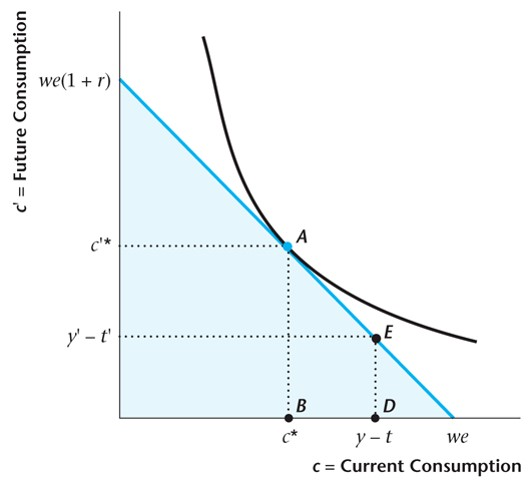
\includegraphics[width=\textwidth]{./figures/Figure9_3.jpg}
            \end{figure}
        \end{column}
        \begin{column}{0.6\textwidth}
            \begin{itemize}
                \item substitute $ c' $: $ \displaystyle \max_{c} U( c, we( 1+r ) - c( 1+r ) ) $
                \item FOC: $ \displaystyle D_{c} U( c, c' ) + D_{c'} U( c, c' ) ( -( 1+r ) ) = 0 $
                \item rearrange: $ \displaystyle \frac{D_{c}U( c, c' )}{D_{c'}U( c, c' )} = \alert{MRS_{c, c'} = 1+r} $
                \item Net worth at pt \textit{E}: excess  endowment at date 0, so saving $ s = y - t - c^{*} > 0 $!
                \item $ c^{*} < y - t $; $ c'^{*} > y' - t'$
            \end{itemize}
        \end{column}
    \end{columns}
\end{frame}

\begin{frame}{Numerical Example}
\label{slide:Numerical_Example}
    \begin{columns}
        \begin{column}{0.5\textwidth}
            \begin{figure}
                \caption{\scriptsize Figure 9.3 A Consumer Who Is a Borrower}
                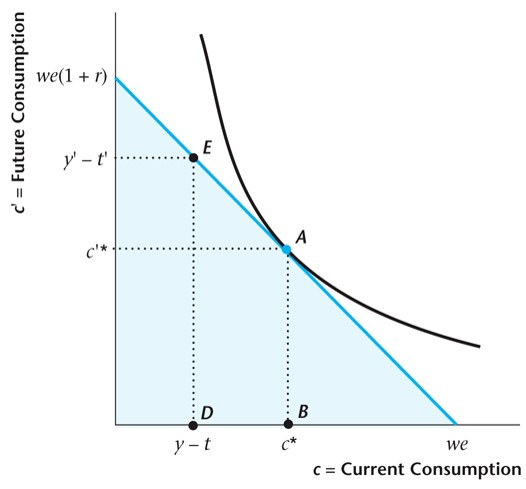
\includegraphics[width=\textwidth]{./figures/Figure9_3_2.jpg}
            \end{figure}
        \end{column}
        \begin{column}{0.5\textwidth}
            Let $ U( c, c' ) = \ln c + \ln c' $ and $ r = 0 $,

            $ \displaystyle MRS_{c, c'} = \frac{1/c}{1/c'} = \frac{c'}{c} = 1+r = 1 $

            optimal bundle: $ c^{*} = c'^{*} $
            \begin{itemize}
                \item if $ we = 1 \Rightarrow c + c' = 1 \Rightarrow c^{*} = c'^{*} = \frac{1}{2}$
                \item if $ E = ( 3/4, 1/4 ) $: consumer saves (last slide)
                \item if $ E = ( 1/4, 3/4 ) $: consumer borrows
            \end{itemize}
        \end{column}
    \end{columns}
\end{frame}

\section{Experiment}
\label{sec:Experiment}

\begin{frame}{Increase in Current income}
\label{slide:Increase_in_Current_income}
    Let consumer's \alert{current} income increases from $ y_1 $ to $ y_{2}$, $ y_{2} > y_{1} $
    \begin{columns}
        \begin{column}{0.5\textwidth}
            \begin{figure}
                \caption{\scriptsize Figure 9.5  The Effects of an Increase in Current Income for a Lender}
                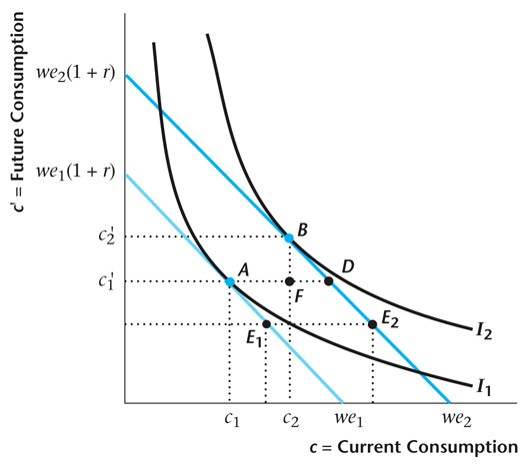
\includegraphics[width=\textwidth]{./figures/Figure9_5.jpg}
            \end{figure}
        \end{column}
        \begin{column}{0.5\textwidth}
            \begin{itemize}
                \item parallel shift in budget line: $ r $ the same
                \item endowment: $ E_{1} $ to $ E_{2} $
                \item optimal bundle: $ A $ to $ B $
                \item consumption smoothing: $c_{1} = c'_{1}$, $c_{2} = c'_{2}$
                \item normality: $ c_{2} > c_{1} $, and $ c'_{2} > c'_{1} $
                \item To support normality, $ s_{2} > s_{1} $
            \end{itemize}
        \end{column}
    \end{columns}
\end{frame}

\begin{frame}{Increase in Future income}
\label{slide:Increase_in_Current_income}
    Let consumer's \alert{future} income increases from $ y'_1 $ to $ y'_{2}$, $ y'_{2} > y'_{1} $
    \begin{columns}
        \begin{column}{0.5\textwidth}
            \begin{figure}
                \caption{\scriptsize Figure 9.8  The Effects of an Increase in Future Income}
                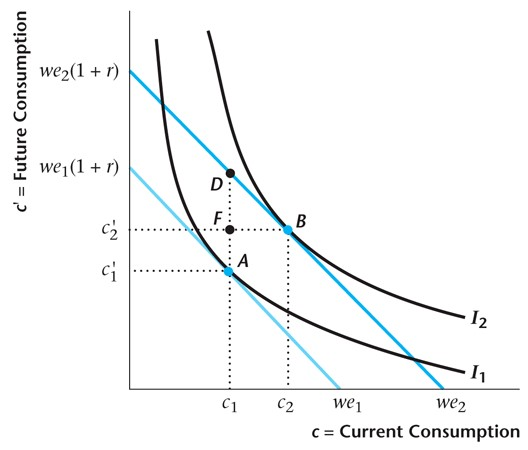
\includegraphics[width=\textwidth]{./figures/Figure9_8.jpg}
            \end{figure}
        \end{column}
        \begin{column}{0.5\textwidth}
            \begin{itemize}
                \item shift in lifetime wealth:
                        $ \displaystyle \Delta we = we_{2} - we_{1} = \frac{y'_{2} - y'_{1}}{1+r} $
                \item optimal bundle: $ A $ to $ B $
                \item consumption smoothing: $c_{1} = c'_{1}$, $c_{2} = c'_{2}$
                \item normality: $ c_{2} > c_{1} $, and $ c'_{2} > c'_{1} $
                \item To support normality, \alert{$ s_{2} < s_{1} $}, shift income from date 1 to date 0!
            \end{itemize}
        \end{column}
    \end{columns}
\end{frame}

\begin{frame}{Intuition: Temporary vs Permanent Change in Income}
\label{slide:Intuition__Temporary_vs_Permanent_Change_in_Income}
    \textbf{Permanent Income Hypothesis} (PIH): changes in income that are permanent have large effects on
permanent income (lifetime wealth) and current consumption.
    \begin{itemize}
        \item temporary change in income: $ y_{1} \rightarrow y_{2}  $ \red{or} $ y'_{1} \rightarrow y'_{2} $
        \item permanent change in income: $ y_{1} \rightarrow y_{2}  $ \alert{and} $ y'_{1} \rightarrow y'_{2} $
        \item intuition: permanent change compounds through lifetime
        \item most of temporary increase saved (e.g. COVID stimulus), yet more permanent increase is consumed (e.g. Rich ppl buys houses)
    \end{itemize}
\end{frame}

\begin{frame}{Visualization: Permanent Income Hypothesis}
\label{slide:Visualization__Permanent_Income_Hypothesis}
    \begin{columns}
        \begin{column}{0.5\textwidth}
            \begin{figure}
                \caption{\scriptsize Figure 9.9  Temporary Versus Permanent Increases in Income}
                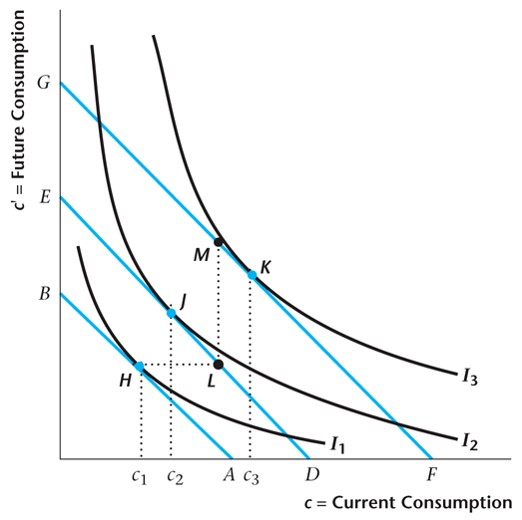
\includegraphics[width=\textwidth]{./figures/Figure9_9.jpg}
            \end{figure}
        \end{column}
        \begin{column}{0.5\textwidth}
            \textbf{Temporary}:
            \begin{itemize}
                \item budget line: $ \overline{AB} \rightarrow \overline{DE} $
                \item optimal bundle: $ H \rightarrow J $
            \end{itemize}
            \textbf{Permanent}:
            \begin{itemize}
                \item budget line: $ \overline{AB} \rightarrow \overline{GF} $
                \item optimal bundle: $ H \rightarrow K $
            \end{itemize}
            In conclusion,
            \begin{itemize}
                \item larger effect on current consumption when change is permanent
                \item temporary $ \Rightarrow  $ saving; not necessary for permanent
            \end{itemize}
        \end{column}
    \end{columns}
\end{frame}

\section{Data}
\label{sec:Data}

\begin{frame}{Consumption Smoothing in Data}
\label{slide:Consumption_Smoothing_in_Data}
    If all consumers act to smooth their consumption relative to their income, then
\alert{aggregate consumption} should likewise be smooth relative to \alert{aggregate income}.
    \begin{itemize}
        \item recall relative volatility: expect $ \sigma_{C}/\sigma_{Y} < 1 $
    \end{itemize}
    There are three main components of aggregate consumption:
    \begin{enumerate}
        \item \textbf{non-durables}: e.g. food, dishes...
        \item \textbf{durables}: e.g. cars, computers...
        \item \textbf{services}: haircuts, repairing...
    \end{enumerate}
    Does our prediction match the data in aggregate consumption? How about prediction with each component?
\end{frame}

\begin{frame}{Durables Behaves Similar to Investment}
\label{slide:Durables_Behaves_Similar_to_Investment}
    \begin{columns}
        \begin{column}{0.5\textwidth}
            \begin{figure}
                \caption{\scriptsize Figure 9.6  Percentage Deviations from Trend in Consumption of Durables and Real GDP, \alert{blue: Durables}, black: GDP}
                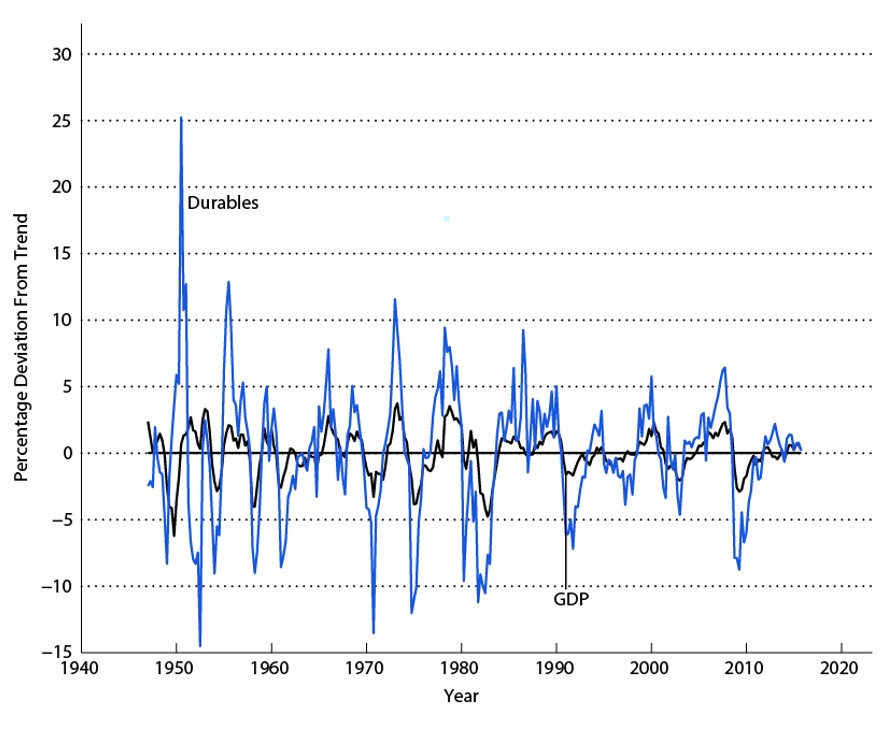
\includegraphics[width=\textwidth]{./figures/Figure9_6.jpg}
            \end{figure}
        \end{column}
        \begin{column}{0.5\textwidth}
            \begin{figure}
                \caption{\scriptsize Figure 3.10 Percentage Deviations from Trend in \alert{Real Investment} and Real GDP, \alert{blue: GDP}, black: investment}
                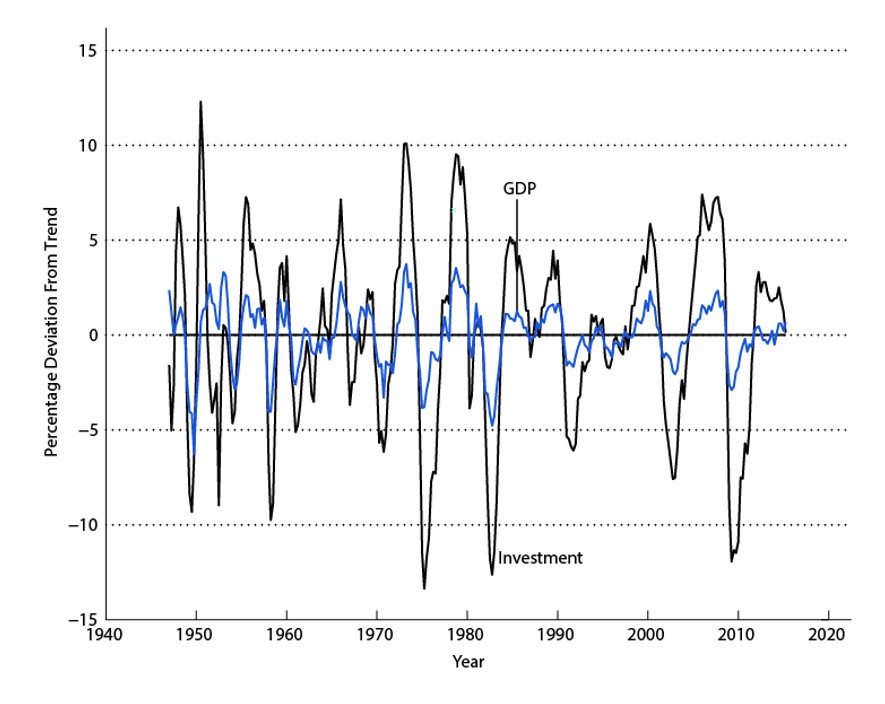
\includegraphics[width=\textwidth]{../Lecture_03/figures/Figure3_10.jpg}
            \end{figure}
        \end{column}
    \end{columns}
\end{frame}

\begin{frame}{Non-Durables \& Services Similar to Agg. Consumption}
\label{slide:Non_Durables_and_Services_Behaves_Similar_to_Agg__Consumption}
\begin{columns}
    \begin{column}{0.5\textwidth}
        \begin{figure}
            \caption{\scriptsize Figure 9.7 Percentage Deviations from Trend in Consumption of Nondurables and Services and Real GDP, \alert{blue: GDP}, \alert{lightblue: Nondurables + Service}}
            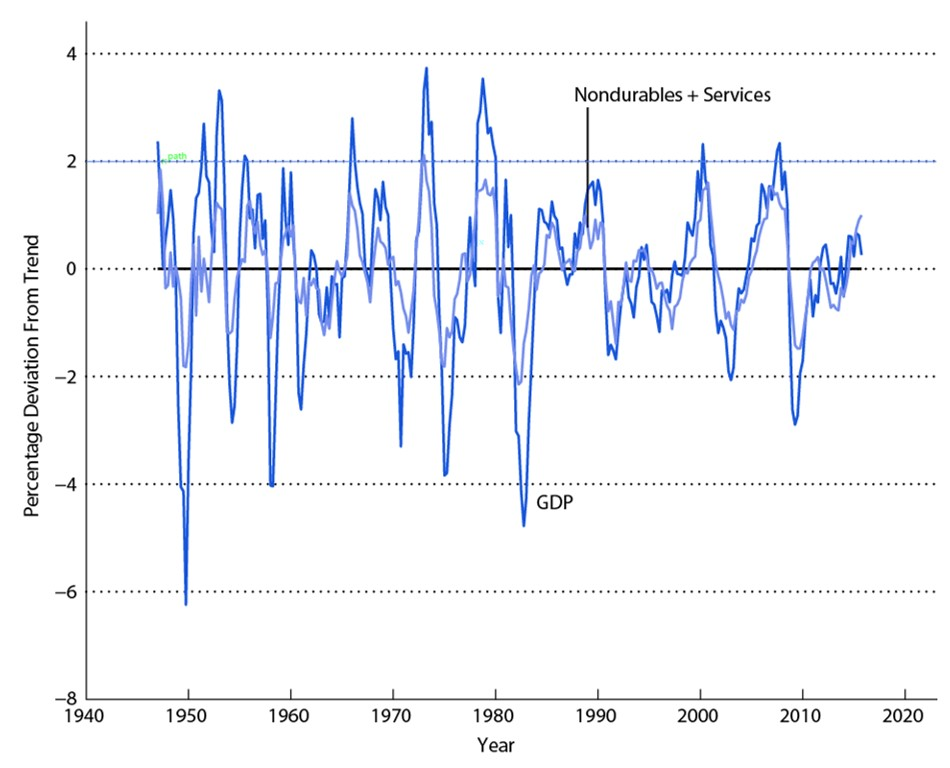
\includegraphics[width=\textwidth]{./figures/Figure9_7.jpg}
        \end{figure}
    \end{column}
    \begin{column}{0.5\textwidth}
        \begin{figure}
            \caption{\scriptsize Figure 3.9 Percentage Deviations from Trend in \alert{Real Consumption} and Real GDP, \alert{blue: GDP}, black: consumption}
            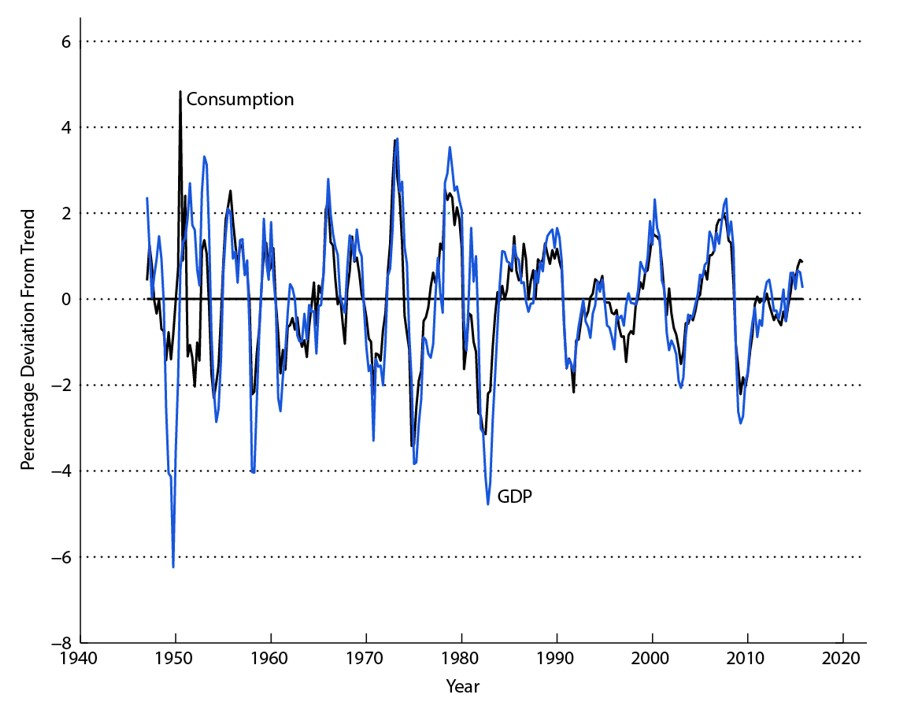
\includegraphics[width=\textwidth]{../Lecture_03/figures/Figure3_9.jpg}
        \end{figure}
    \end{column}
\end{columns}
\end{frame}

\end{document}

